
\documentclass[12pt]{article}
\usepackage[english]{babel}
\usepackage[utf8x]{inputenc}

\usepackage{amsmath}
\usepackage{graphicx}
\usepackage[colorinlistoftodos]{todonotes}
\usepackage{caption}
\usepackage{hyperref}
\usepackage{float}
\usepackage{subfig}
\usepackage{comment}
\usepackage{subcaption}
\usepackage{multirow}
\usepackage{listings}
\usepackage{indentfirst}
\definecolor{codegreen}{rgb}{0,0.6,0}
\definecolor{codegray}{rgb}{0.5,0.5,0.5}
\definecolor{codepurple}{rgb}{0.58,0,0.82}
\definecolor{backcolour}{rgb}{0.95,0.95,0.92}
 \usepackage{tikz}
 \usepackage{pifont}
\usepackage{makecell}
\usepackage{adjustbox}
\usepackage{enumitem}
\usetikzlibrary{trees}
\lstdefinestyle{mystyle}{
    backgroundcolor=\color{backcolour},   
    commentstyle=\color{codegreen},
    keywordstyle=\color{magenta},
    numberstyle=\tiny\color{codegray},
    stringstyle=\color{codepurple},
    basicstyle=\footnotesize,
    breakatwhitespace=false,         
    breaklines=true,                 
    captionpos=b,                    
    keepspaces=true,                 
    numbersep=5pt,                  
    showspaces=false,                
    showstringspaces=false,
    showtabs=false,                  
    tabsize=2
}
\lstset{style=mystyle}
\usepackage{titlesec}
\titleformat{\paragraph}
{\normalfont\normalsize\bfseries}{\theparagraph}{1em}{}
\titlespacing*{\paragraph}
{0pt}{3.25ex plus 1ex minus .2ex}{1.5ex plus .2ex}
\begin{document}


\begin{titlepage}


\newcommand{\HRule}{\rule{\linewidth}{0.5mm}} % Defines a new command for the horizontal lines, change thickness here

\center % Center everything on the page
 
%----------------------------------------------------------------------------------------
%	HEADING SECTIONS
%----------------------------------------------------------------------------------------

\textsc{\LARGE Universidade de Aveiro}\\[1.5cm] % Name of your university/college
\textsc{\Large IEETA}\\[0.5cm] % Major heading such as course name
\textsc{\Large RETIOT}\\[0.5cm]

%----------------------------------------------------------------------------------------
%	TITLE SECTION
%----------------------------------------------------------------------------------------

\HRule \\[0.4cm]
{ \huge \bfseries Technical Report}\\[0.4cm] % Title of your document
\HRule \\[1.5cm]
 
%----------------------------------------------------------------------------------------
%	AUTHOR SECTION
%----------------------------------------------------------------------------------------

\begin{minipage}{0.4\textwidth}
\begin{flushleft} \large
Francisco Santos % Your name
\end{flushleft}
\end{minipage}
~
\begin{minipage}{0.4\textwidth}
\begin{flushright} \large
Nº76618\\
\end{flushright}
\end{minipage}\\[2cm]

% If you don't want a supervisor, uncomment the two lines below and remove the section above
\Large {RETIOT -}
%John \textsc{Smith}\\[3cm] % Your name

%----------------------------------------------------------------------------------------
%	DATE SECTION
%----------------------------------------------------------------------------------------

{\large \emph{February de 2018}}\\[2cm] % Date, change the \today to a set date if you want to be precise

%----------------------------------------------------------------------------------------
%	LOGO SECTION
%----------------------------------------------------------------------------------------


\includegraphics[scale=0.4]{ua_logo.png} % Include a department/university logo - this will require the graphicx package
 
%----------------------------------------------------------------------------------------

\vfill % Fill the rest of the page with whitespace

\end{titlepage}
%%\renewcommand{\figurename}{Figura}
%%\renewcommand{\tablename}{Tabela}
%%\renewcommand{\contentsname}{Conteúdo}
\tableofcontents
\newpage

\section{Introduction}
The focus of this report is to present and explain the various tasks fulfilled in the scope of the project \textbf{RETIOT, “Reflectometry Technologies to Enhance the Future Internet of Things and Cyber-Physical Systems"}. The main objective is to interface the \textit{Texas Instruments mmwave} radar sensor with the \textit{Robot Operating System} and use it to achieve autonomous navigation for the \textbf{turtlebot2} robot.


\section{Procedure}
In order to achieve our objectives the work was split in the following tasks:
\begin{enumerate}
    \item Familiarization with the Robot Operating System.
    \item Create an interface between TI mmwave devices and ROS.
    \item Process the retrieved data in order to  accommodate our application.
    \item Understand the ROS navigation stack architecture and parametrization.
    \item Using ROS navigation stack with both radar and lidar sensor information to achieve fully autonomous navigation for the \textbf{turtlebot2} robot.
\end{enumerate}
\section{Robot Operating System}

\subsection{Introduction}
Robot Operating System (ROS) is an open-source, meta-operating system that provides libraries and tools to help developers create robotic applications. This includes hardware abstraction, device drivers, tools for introspection, message-passing and more.
\subsection{ROS architecture}
%MORE STUFF
The ROS structure is composed by:
\begin{itemize}
\item \textbf{Nodes} - Processes that perform computation.
\item \textbf{Messages} - ROS predefined data type used to communicate between nodes. 
\item \textbf{Topics} - Nodes can send messages by publishing to a topic or receive them by subscribing to a topic. 
\item \textbf{Master} - Provides registration of names (helps nodes find each other).
% V
\item \textbf{rosout} - ROS equivalent of stdout 
\item \textbf{roscore} - Master+rosout+parameter server. 
%X
\end{itemize}
%%\subsubsection{ROS nodes}
%%\subsubsection{ROS topics}
%%\subsubsection{ROS subscribers and publishers}
%%REVER ISTO

Figure \ref{fig:ros_concepts} shows an overview of the general architecture of ROS.

\begin{figure}[!htb]
    \centering
    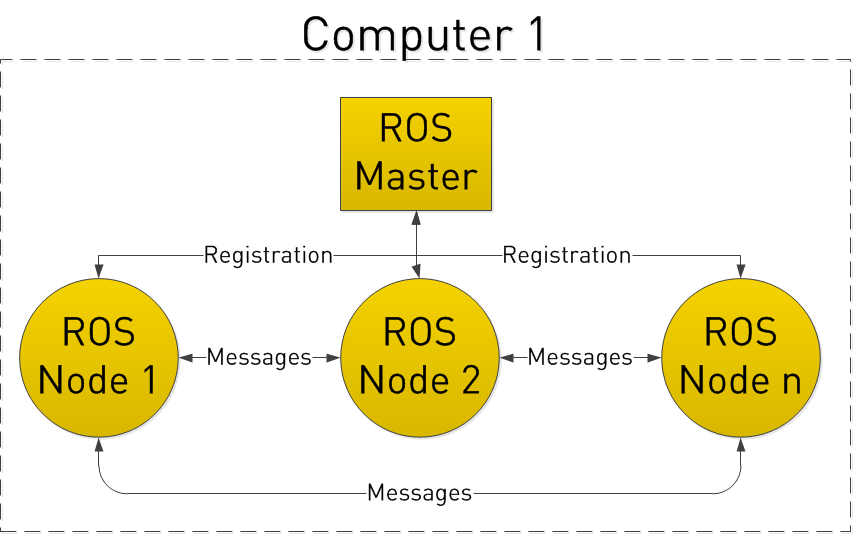
\includegraphics[scale=0.28]{ros_graph.png}
    \caption{ROS architecture overview}
    \label{fig:ros_concepts}
\end{figure}
\section{Interface between ROS and the radar}
Texas Instruments provides a ros package that interfaces radar data to the ROS message format. The incoming radar data from the mmWave EVM is decoded in order to create a \textbf{PointCloud2} type ROS message which is published in topic \textbf{/radar/RScan}.

\subsection{PointCloud2 radar data stucture}

%%PUT figure:
The published ROS message PointCloud2 follows the mmwave demo structure (Fig. 2). Each point has 6 fields:
\begin{itemize}
\item x - position x of the detected  object in the frame of the radar.
\item y - position y.
\item z - position z (for 2D devices this is equal to zero).
\item range - range of the object relative to the radar frame.
\item doppler - radial velocity of the object relative to the radar frame.
% POR IMAGEM
\item intensity - relative power of the received signal corresponding to that object.
\end{itemize}

\begin{figure}[!htb]
    \centering
    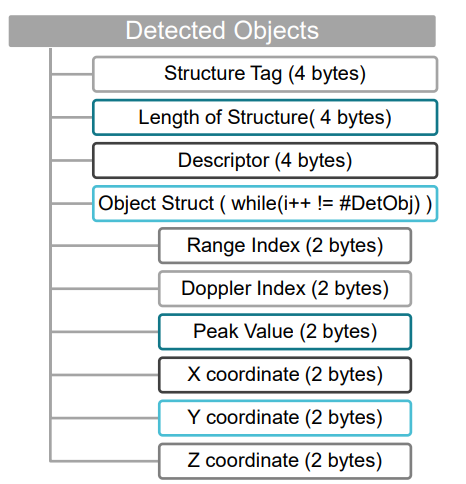
\includegraphics[scale=0.5]{2_demo_vis_struct.PNG}
    \caption{Part of the mmwave demo packet containing object detection information. This fields will be used to construct the ROS PointCloud2.}
    \label{fig:my_label}
\end{figure}
\subsubsection{Running the driver and observing the outputted pointcloud in rviz}
To start receiving and visualizing the incoming radar data run the following commands while in your ROS workspace directory:
 \begin{lstlisting}[language=bash]
source devel/setup.bash
roslaunch ti_mmwave_rospkg rviz_1642_2d.launch
\end{lstlisting}
This will launch the TI mmWave ROS Driver nodes that configure the EVM and publish the radar data. After that rviz will load and you should be able to visualize the objects detected by the radar. Figure \ref{fig:radar_rviz} shows an example of the radar data displayed on rviz. The points correspond to object detected by the radar.

\begin{figure}[!htb]
    \centering
    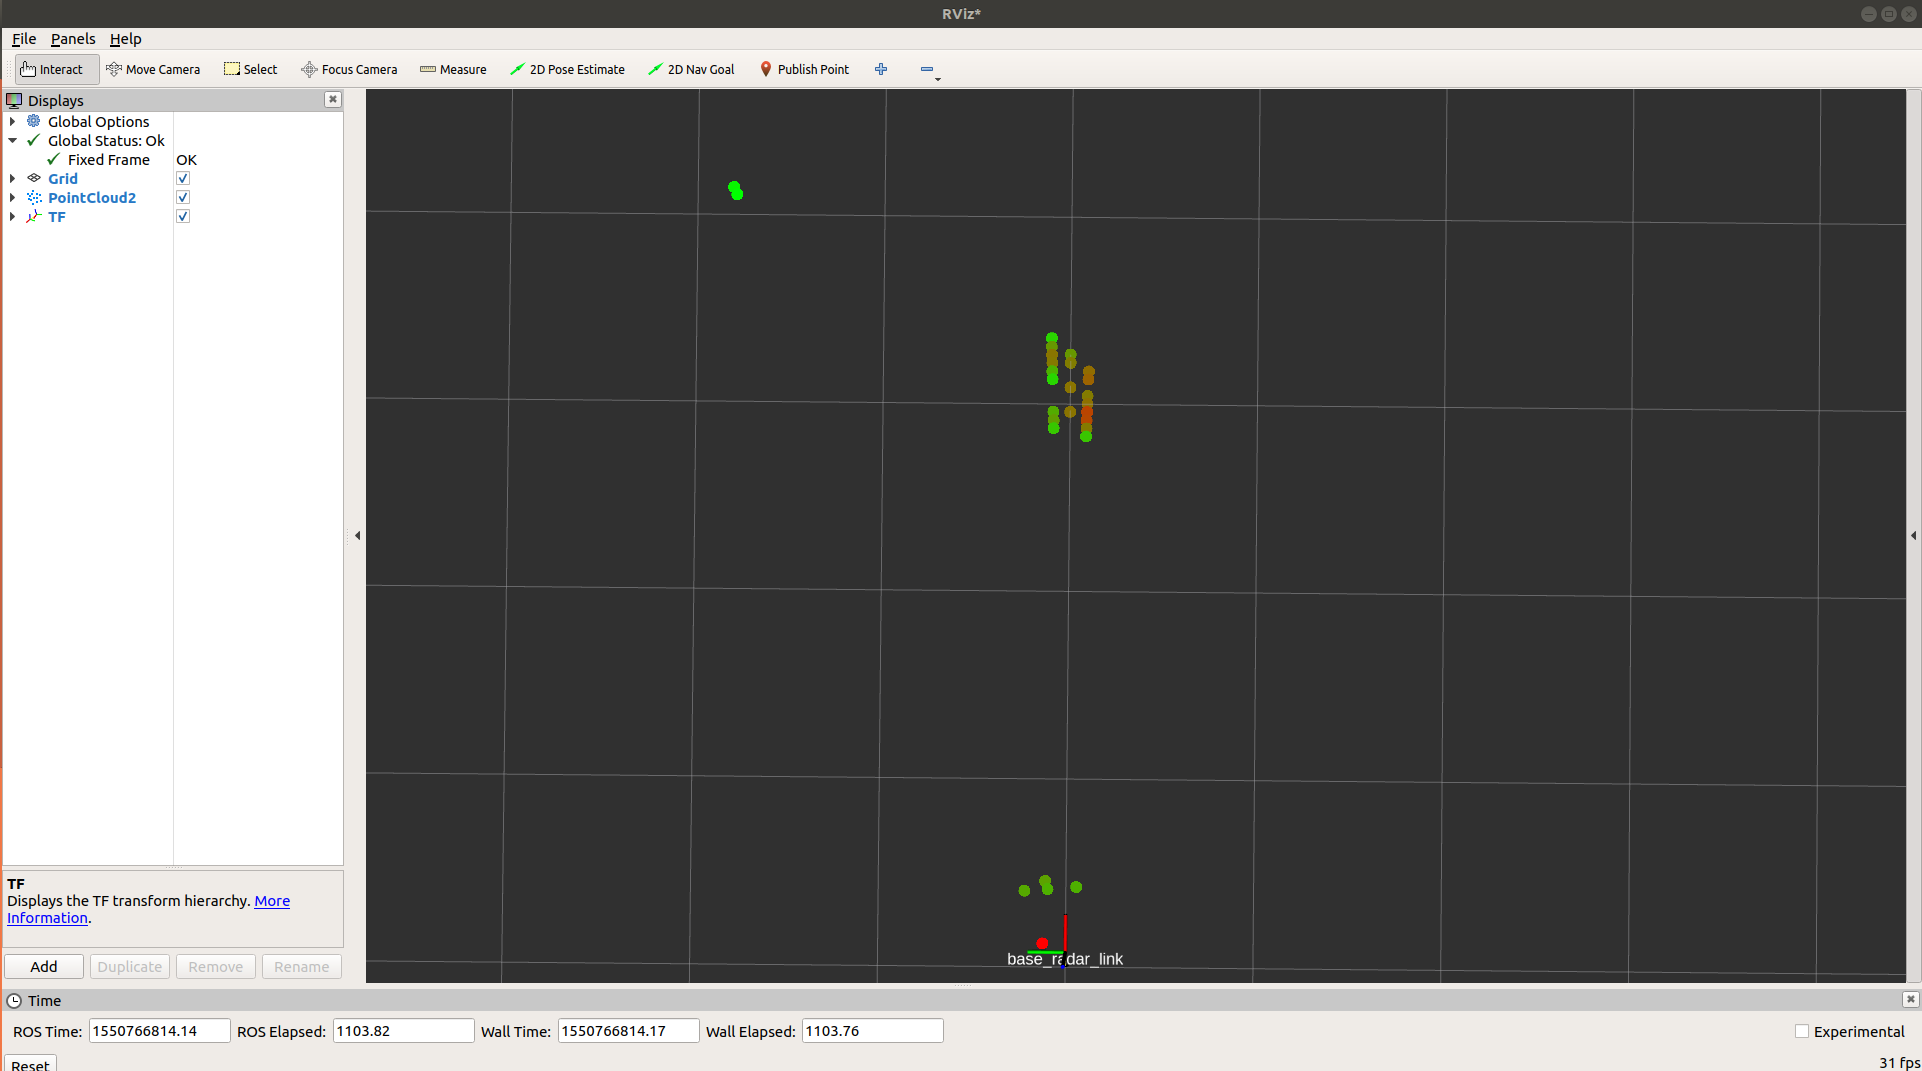
\includegraphics[scale=0.2]{pc_not_filt.png}
    \caption{Pointcloud2 radar data displayed by rviz}
    \label{fig:radar_rviz}
\end{figure}
\subsection{Visualization of the radar point cloud}
Plotting the points in the XYZ space is not enough to fully visualize the radar data sent since each point also gives velocity and intensity information.
We can visualize it by using markers such as arrows or text in rviz.
Figure \ref{fig:doppler_marker} displays the radial velocity of each point with an arrow. The size of the arrow indicates how fast the object is going. Figure \ref{fig:intensity_marker} shows the intensity values of each object in text. This type of visualization will be useful later on when we try to filter the cloud.

\begin{figure}[!htb]
    \centering
    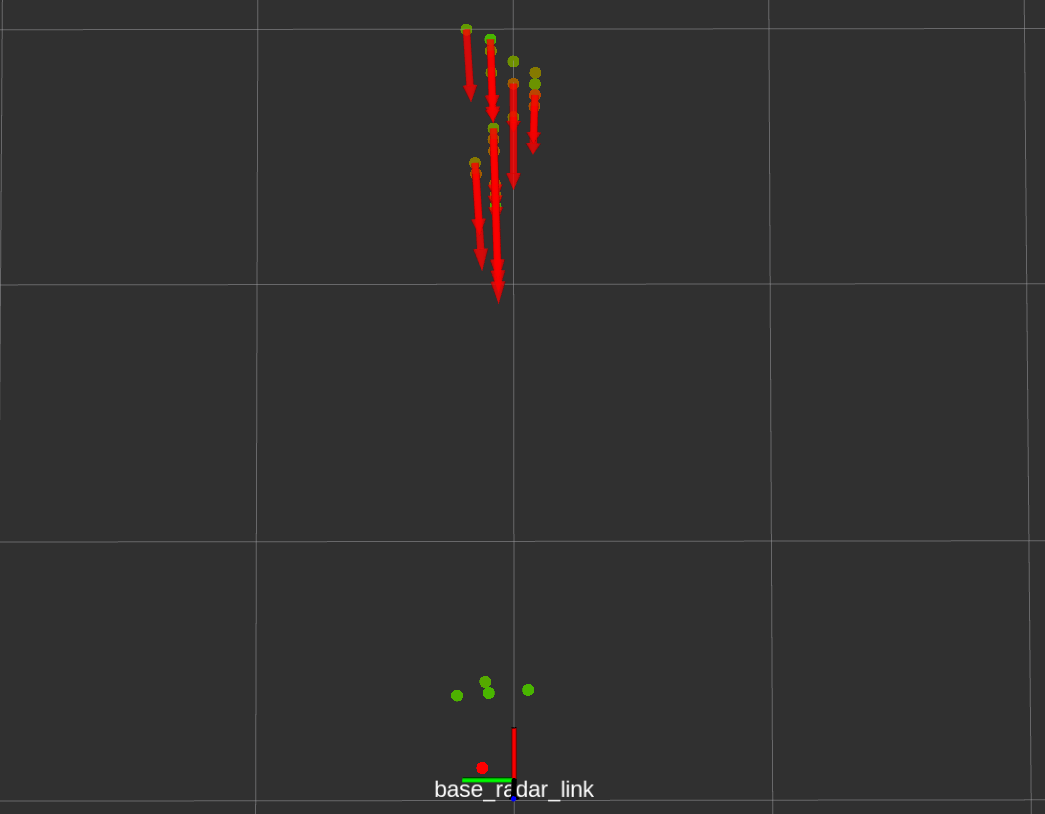
\includegraphics[scale=0.25]{doppler_marker.png}
    \caption{Arrow markers displaying the points radial velocity}
    \label{fig:doppler_marker}
\end{figure}

\begin{figure}[!htb]
    \centering
    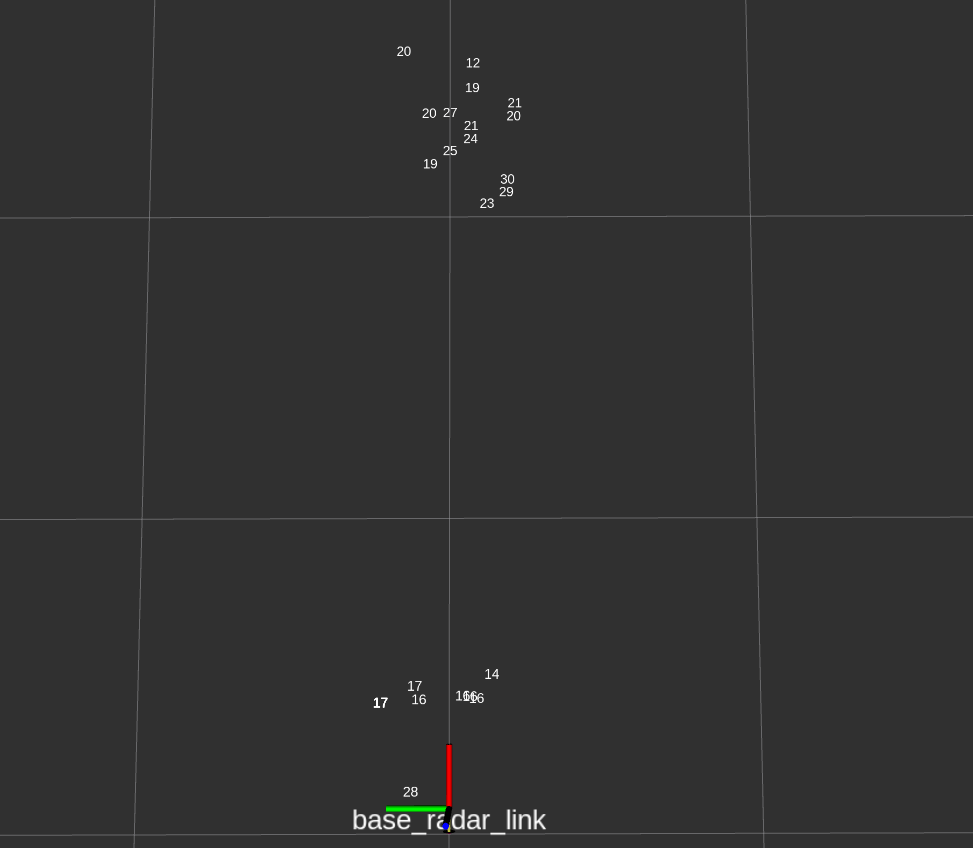
\includegraphics[scale=0.25]{intensity_marker.png}
    \caption{Text markers displaying the points intensity values}
    \label{fig:intensity_marker}
\end{figure}
\subsection{Chirp profile configuration file}
The characteristics of this point cloud such as publishing rate, range resolution, maximum range, velocity resolution, maximum velocity depends on the chirp profile configuration file loaded in the EVM. This file is located in the \textbf{"cfg"} folder of the ti mmwave package and can be replaced in order to accommodate a given application.

The easiest way to create a chirp configuration file is the mmWave Demo Visualizer. With it you can auto generate a configuration file given a set of specifications.
Another way of doing this is manually. This however requires the understanding of the radar operating principle and the meaning of the commands in the configuration file.
%??????????????
%For more information on this topics we suggest the reading of the links bellow:
%SDK USER GUIDE
%CHIRP PARAMETER CONFIG

\section{Radar Data Processing}
Now that we have the radar constantly giving us a point cloud we can further process to retrieve the information we want. 
In our case we will make use of \textbf{passthrough filters} to remove unwanted points and \textbf{euclidean clustering} to identify groups of points that belong to the same object.

This operations will be done by using the \textbf{Point Cloud Library}. PCL offers a wide variety of modules that handle point clouds but in our case we will only use it for the previously mentioned operations.
%PCL NO FIM
\subsection{Passthrough Filters}
In the point cloud there may be some points that have undesirable characteristics, such as points with low intensity  that lead to false detections or outside of the radar operating range. To remove this points we use \textbf{passthrough filters} that specify the range of values a given field can have in order for a point to be kept in the point cloud. 

For example, if we are only interested in obstacles that are moving between 0.5 m/s and 1.0 m/s (radial velocity), this can be done by using a pass through filter on the doppler channel.
Figure \ref{fig:filters} shows an example where we delete false detections close to the radar by filtering the pointcloud by intensity.
\begin{figure}[h]%
    \centering
    \subfloat[Non filtered pointcloud]{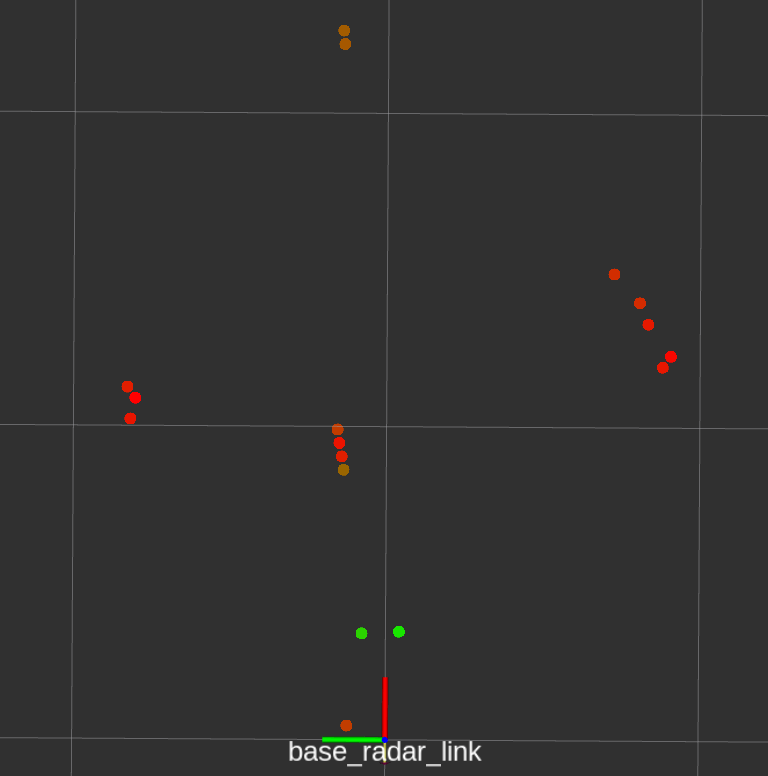
\includegraphics[width=6.34cm]{not_filt.png} }%
    \qquad
    \subfloat[Filtered pointcloud by intensity]{{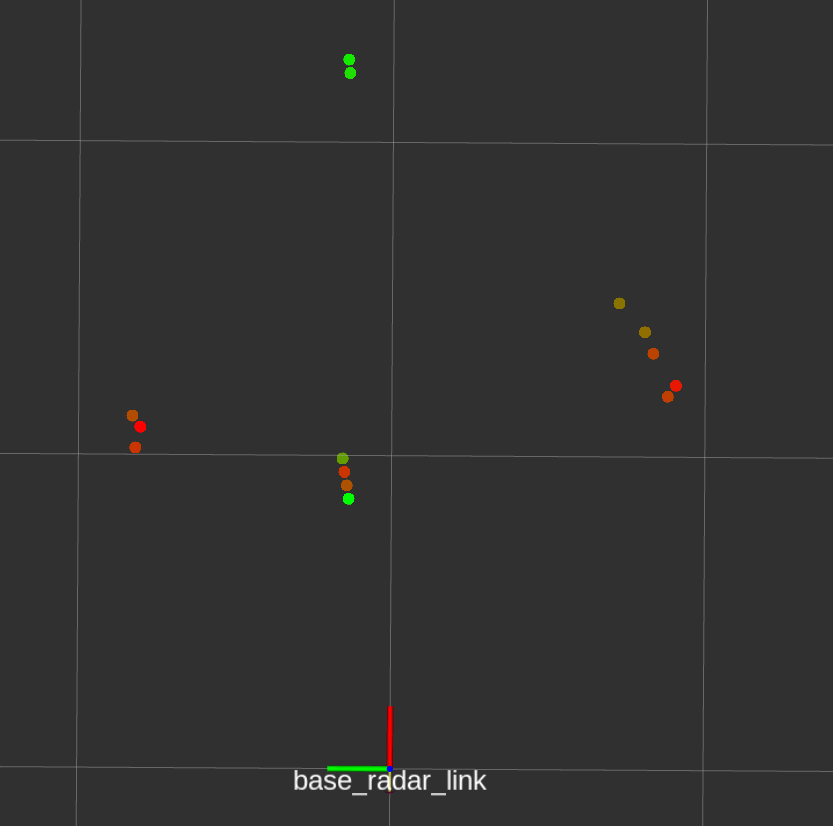
\includegraphics[width=6.34cm]{filt.png}}}%
    \caption{Example of filtering the pointcloud}%
    \label{fig:filters}
\end{figure}

%%PUT IMAGE INTENSITY FILTERING  RVIZ
\subsection{Euclidean Clustering}
%Objectivos do clustering
To identify objects such as persons we can use euclidean clustering. This identifies a subset of points that are close together. The two main parameters in this operation are:
\begin{itemize}
\item \textbf{minClusterSize} - Minimum number of points a cluster must have in order to be valid.
\item \textbf{ClusterTolerance}  - Maximum distance a point may have to a cluster member to also be counted as member of that cluster.
\end{itemize}
%%%PUT CLUSTER RVIZ FIGURE
This parameters must be tuned to the type of cluster we want to find. 
If the \textbf{ClusterTolerance} parameter is too small, it can happen that an actual object can be seen as multiple clusters, if the value is high, it could happen that multiple objects are seen as one cluster.
%In figure \ref{fig:filters} we use the module pcl
%% CLUSTER FIGURE
\begin{figure}[!htb]
    \centering
    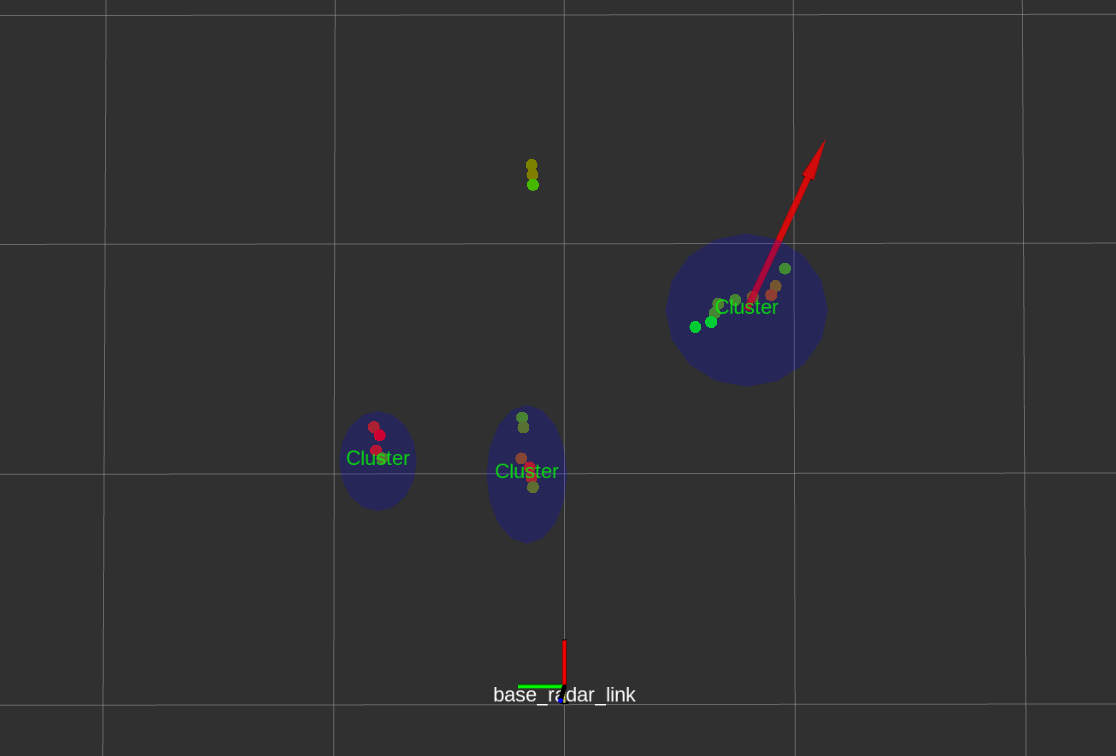
\includegraphics[width=\linewidth]{cluster.png}
    \caption{Clusters found on the radar pointcloud}
    \label{fig:clustering}
\end{figure}
\subsection{Using radar velocity information to predict cluster movement}
We previously said that our point cloud has a doppler channel that retrieves the relative radial velocity of the point in respect to the radar. We can use this information to compute the mean velocity of a cluster and make a prediction of its position in the future. This comes with the limitation that the radar only gives us radial velocity so the prediction will just estimate if the cluster will be closer or further away. 
However this information might be useful later on when we want to avoid collisions with incoming moving objects when our robot is navigating.


%%PUT IMAGE OF PREDICTED PC2
\section{ROS navigation stack}
%Less Implementation More general explaining of how to navigate
The ROS navigation stack is a set of software packages that properly combined can get a robot to navigate autonomously.
Figure X  shows an example of turtlebot2 using the navigation stack to drive in rviz.
However, before running it we first need to properly setup the robot.
\subsection{Requirements}
\subsubsection{Transform Configuration}
The Navigation stack requires that the relationships between the different frames must be published in \textbf{tf} or \textbf{tf\_static} topic. This makes it so the robot perceives what is around him correctly.
Figure \ref{fig:tf} shows all the frames and their transforms with each other for \textbf{turtlebot2}. However the main transforms we need to worry about are between the sensors and the base link frame.
\begin{figure}[!htb]
    \centering
    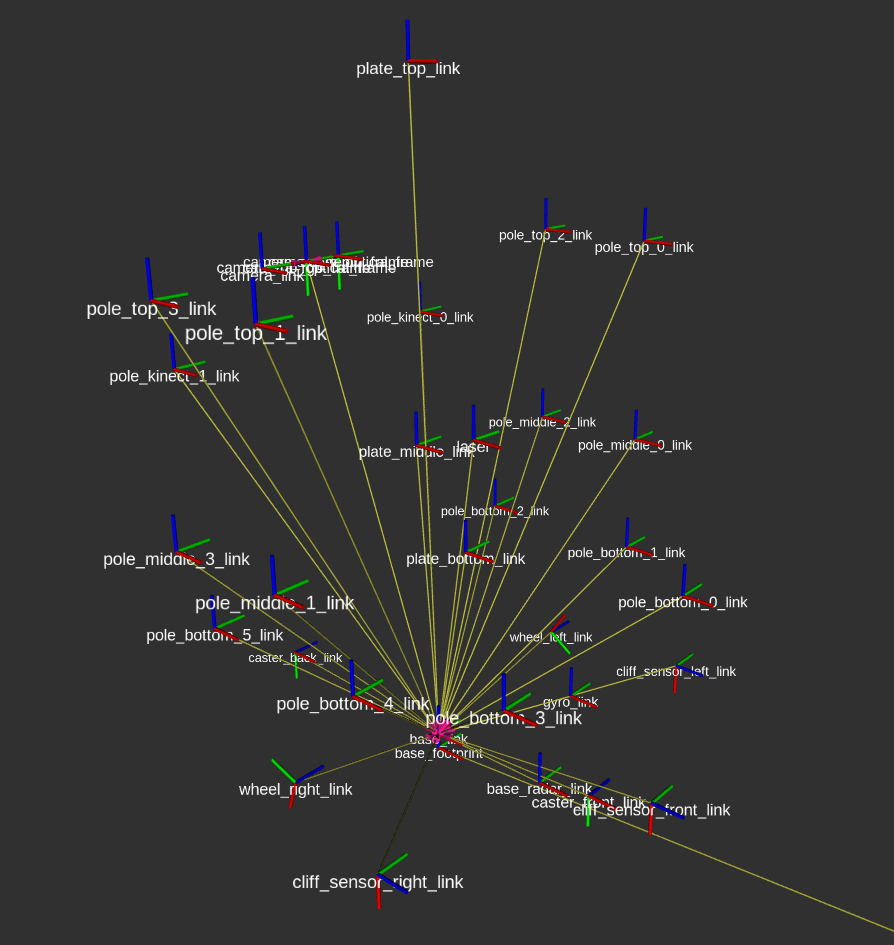
\includegraphics[scale=0.2]{tf.png}
    \caption{Transform relationships in our robot}
    \label{fig:tf}
\end{figure}
\subsubsection{Sensor sources}
To avoid obstacles we need some type of sensors that can detect them. Before running the stack we need to make sure they are publishing this information.
%in the \textbf{PointCloud2} or \textbf{LaserScan} ROS message format
In our case we will use both the \textbf{radar} (PointCloud2) and the \textbf{lidar} (LaserScan) as our observation sources.
Figure \ref{fig:sensors} shows an example of the published data from both in rviz.
\begin{figure}[!htb]
    \centering
    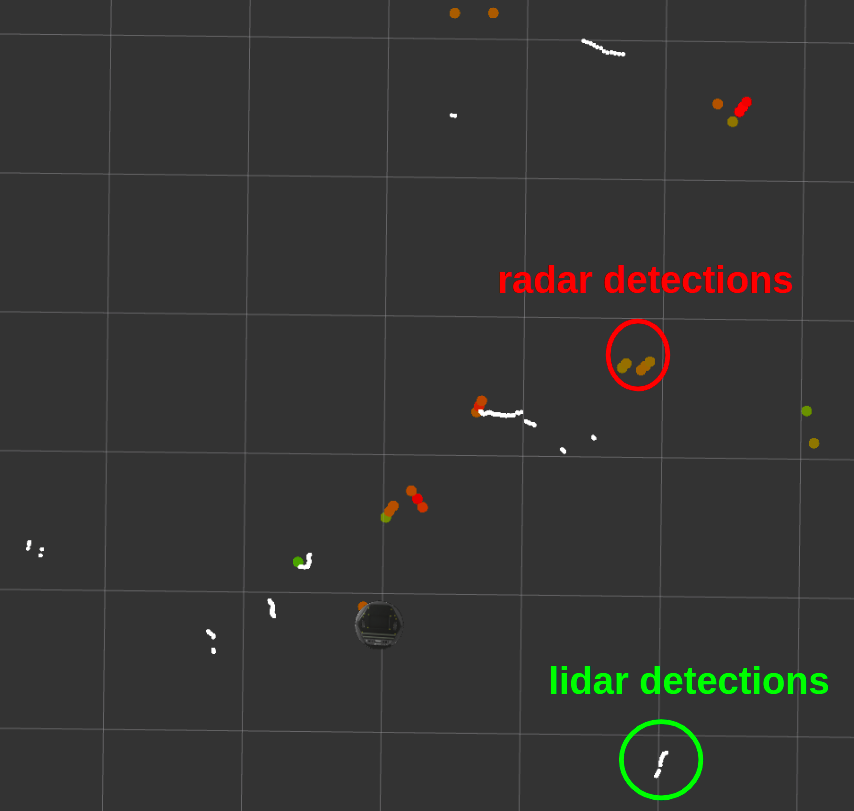
\includegraphics[scale=0.2]{sensors2.png}
    \caption{Obstacle defections by both radar and lidar}
    \label{fig:sensors}
\end{figure}
\subsubsection{Odometry}
We need to localize the robot in some way to correctly navigate. Therefore we require a topic that publishes odometry information.
%%AMCL
\subsubsection{Base Controller}
This node will subscribe to the velocity message outputted by the navigation stack and convert them into the appropriate motor commands to send to the mobile base that will actually make the robot move.

\subsubsection{Mapping}
This part is not mandatory but it helps to have a some sort of map being published to use as a global reference for the robot. It is used by \textbf(amcl) to correctly localize the robot and to mark previously detected lethal obstacles when the map was built. Fig. \ref{fig:map} shows an example of a map that might be used by the ROS navigation stack.
\begin{figure}[!htb]
    \centering
    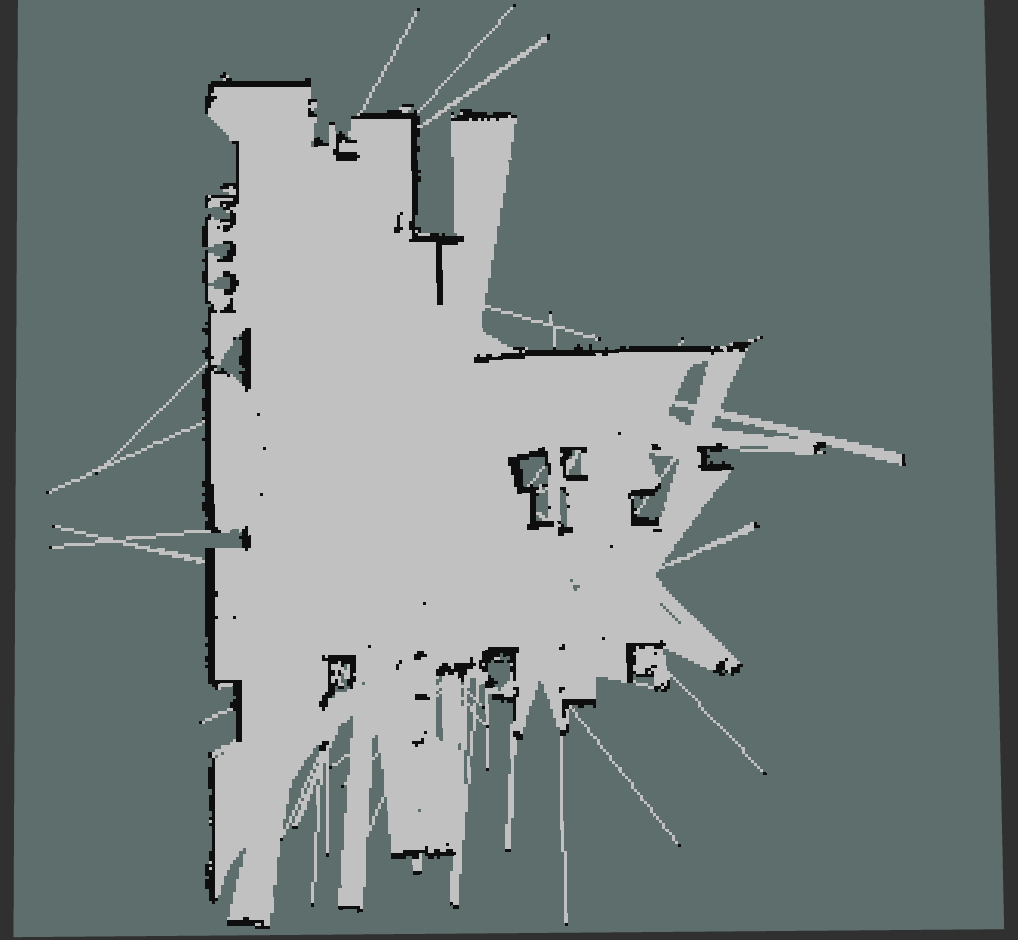
\includegraphics[scale=0.2]{map.png}
    \caption{Example of a map created in the IRIS laboratory}
    \label{fig:map}
\end{figure}


If the setup is done correctly we can now run the navigation stack.
\subsection{Navigation Stack components}
%%STUFF
Now that we have all the things we need for navigation we need an entity that actually processes all this information in an intelligent way to determine the best velocity command for the robot. This is done by the \textbf{move\_base node} and its peripherals.
Figure \ref{fig:plans} shows an example of the global and local plan calculated by the ROS navigation stack.
\begin{figure}[!htb]
    \centering
    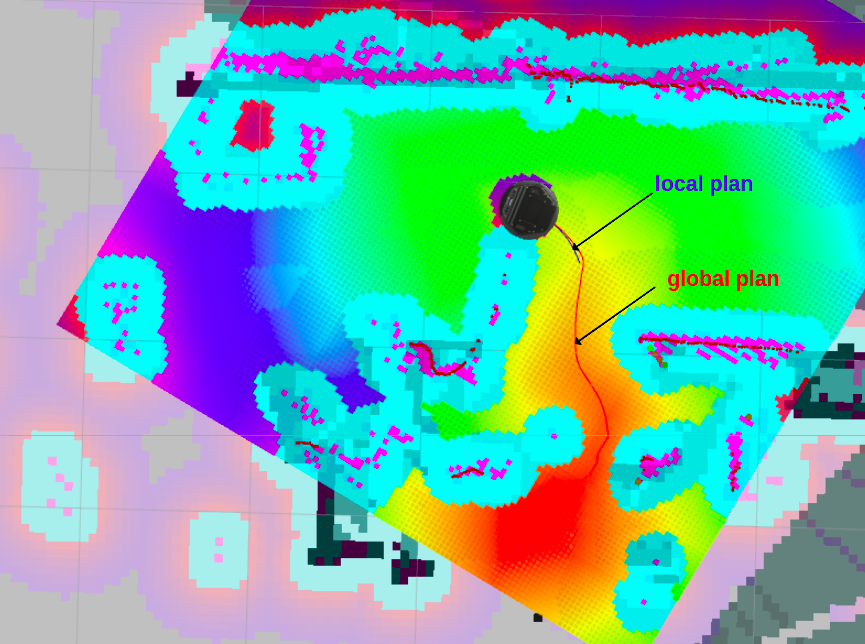
\includegraphics[width=\linewidth]{rviz_navigation2.png}
    \caption{Global and Local plan calculated by the navigation stack}
    \label{fig:plans}
\end{figure}
\subsubsection{Move Base}

The move base node base links together a global and local planner as well as a local and global costmap to achieve the end goal provided by an action server. It also loads a set of determined recovery behaviors if the planners fail to produce a valid path. 

The global and local planners are plugins specified by the user. This choice will affect the behavior of the robot depending on the planners architecture and parameters. 

\subsubsection{Global Planner}
 
The job of this component is to produce the best trajectory for a robot to take with limited amount of information given by the global costmap.
This plan can be updated when the robot gets stuck or by a user specific frequency (\textbf{planner\_frequency}). The algorithms used to get this path are usually \textbf{dijaktra} or \textbf{A*}.

\subsubsection{Local Planner}
The local planner takes into account the trajectory given by the global planner and tries to compute velocity commands that follow it. However the path given may be to close to an obstacle detected and in order to avoid it we must deviate from the plan given to avoid collision. The function of the local planner is to avoid dynamic obstacles that appear while still trying to follow the global plan and goal. 

\subsubsection{Local and Global Costmap}
The global and local costmap share the same class, the  \texttt{Costmap2DROS}. This class consists of a layered costmap that takes into account various layers defined by the user.

\paragraph{Available Layers}
\begin{itemize}[label={}]
    \item \textbf{Obstacle Layer} - Marks objects retrieved from \texttt{observation\_sources} with lethal value. It also raytraces observations to clear out space.
    %Does more stuff
    \item \textbf{Inflation Layer} - Inflates the detected obstacles taking into account the \texttt{robot\_radius} and \texttt{inflation\_radius}. The closer the cells are from a lethal obstacle the more value they will have.
    %%....(needs explanation)
    \item \textbf{Static Layer} - Retrieves static information from the \textbf{/map} topic and marks them has lethal objects (Typically only used in global costmap).
\end{itemize}
Figure \ref{fig:layers} shows how the combined layers produce the master costmap that will be used by the planners.
\begin{figure}[!htb]
    \centering
    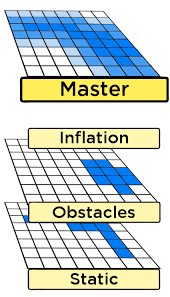
\includegraphics{layers.png}
    \caption{Different layers used to create the final costmap grid that will be used in the navigation stack}
    \label{fig:layers}
\end{figure}
All the user defined layers will in conjunction create the final master costmap (either local or global) that will be used by the planners.


\subsection{Navigation Stack Parameters}
In this section it is presented and described the main parameters of each component of the navigation stack. It also explains the impact they will have on the robot's behavior when navigating.

Some parameters are omitted due to being less relevant in this context and should be considered as having the default value.
\subsubsection{Move Base}
The \textbf{move\_base} node is responsible for organizing the communications between all the stack components and managing the state of the robot.
\paragraph{Main Parameters}
\begin{itemize}[label={}]
    \item \texttt{controller\_frequency $(Hz)$} - Frequency at which move base will ask the local planner for velocity commands.
    \item \texttt{controller\_patience $(s)$} - Maximum amount of time to get a valid velocity from the local planner before going to recovery behavior.
    \item \texttt{planner\_frequency $(Hz)$} - Frequency at which the move base will ask the global planner for a new plan. If set to 0.0 it will only update the plan when the robot gets stuck.
    \item \texttt{planner\_patience $(s)$} - Maximum amount of time to get a valid global plan before going to recovery behavior (only if its in PLANNING state).
\end{itemize}

Increasing the \texttt{controller\_frequency} and \texttt{planner\_frequency} parameters will improve the overall responsiveness of the robot. However it demands a higher computational power that the robot might not have and will result in the loops missing their desired rates.
%%PUT GOOD VALUES?

The \texttt{controller\_patience} and \texttt{planner\_patience} parameters will determine the tolerance for the global and local planner to produce valid plans and velocities. If you want the robot to express recovery behaviors quickly when it gets stuck you should decrease this parameters. If you want to give the robot more time to think than increase them instead.

\subsubsection{TrajectoryPlannerROS}

\textbf{TrajectoryPlannerROS} is encharged of computing the velocity that will be sent to the mobile base. To do this it simulates various velocities, calculates the associated trajectories for a given time and picks the one with lowest cost. The cost is determined by the \textbf{cost function} that takes into account the local goal, the global plan and local costmap values in the trajectory points.

\paragraph{Main Parameters}
\begin{itemize}[label={}]
    \item \texttt{acc\_lim\_x $(m/s²)$} - x (translation) acceleration limit.
    \item \texttt{acc\_lim\_theta $(radians/s²)$} - rotational acceleration limit.
    \item \texttt{max\_vel\_x $(m/s)$} - x maximum allowed velocity.
    \item \texttt{min\_vel\_x $(m/s)$} - x minimum allowed velocity.
    \item \texttt{max\_vel\_theta $(radians/s)$} - maximum allowed rotational  velocity.
    \item \texttt{min\_vel\_theta $(radians/s)$} - minimum allowed rotational velocity.
    \item \texttt{sim\_time $(s)$} - The amount of time to forward-simulate trajectories.
    \item \texttt{vx\_samples} - number of samples in the x velocity space to use in the simulation.
    \item \texttt{vtheta\_samples} - number of samples in the theta velocity space to use in the simulation.
    \item \texttt{pdist\_scale} - Weight for how much the trajectory should be close to the global plan.
    \item \texttt{gdist\_scale} - Weight for how much the trajectory should be close to the local goal.
    \item \texttt{occdist\_scale} - Weight for how much the trajectory should avoid obstacles.
\end{itemize}

The velocity and acceleration limits should be set to choose  less than the base's capability to ensure the computed velocities are actually physically achievable. In the \textbf{turtlebot2} case, its maximum  translational velocity is 0.7 m/s and its maximum rotational velocity is 180 deg/s (3.14 rad/s).

\paragraph{Getting the Best Trajectory}
The algorithm to get the best trajectory goes as follows:
\begin{enumerate}
    \item Discreetly sample the velocity space ($d_{vx}$ and $d_{vtheta}$)
    \begin{align*}
        & d_{vx}=(\texttt{max\_vel\_x}-\texttt{min\_vel\_x})/\texttt{vx\_samples}\\
         & d_{vtheta}=(\texttt{max\_vel\_theta}-\texttt{min\_vel\_theta})/\texttt{vtheta\_samples}
    \end{align*}
    \item For each sampled velocity predict its trajectory in a given time frame (\texttt{sim\_time}).
    \item Evaluate the cost of each trajectory  by using the value cost function
    \item Pick the one with lowest cost and publish the associated velocity.
    \item Repeat for a given rate (\texttt{controller\_frequency})
\end{enumerate}

%%SIMULATION IMAGE
%%SIM TIME S
\paragraph{Cost Function}
The cost function used to evaluate a trajectory is given by:
\begin{align*}
        \textbf{cost} = &
   \texttt{pdist\_scale} * \textbf{path\_dist}
   + \texttt{gdist\_scale} * \textbf{goal\_dist}\\
   &+\texttt{occdist\_scale} * \textbf{maxobscost} 
\end{align*}

Where \textbf{path\_dist} is the distance from the endpoint of the trajectory to the global path in map cells or meters, \textbf{goal\_dist} is the distance from the endpoint of the trajectory to the local goal in map cells or meters and \textbf{maxobscost} is equal to the \textbf{maximum obstacle cost} (given by the local costmap) of all the points along the trajectory.



%%RVIZ cost cloud
\begin{figure}[!htb]
    \centering
    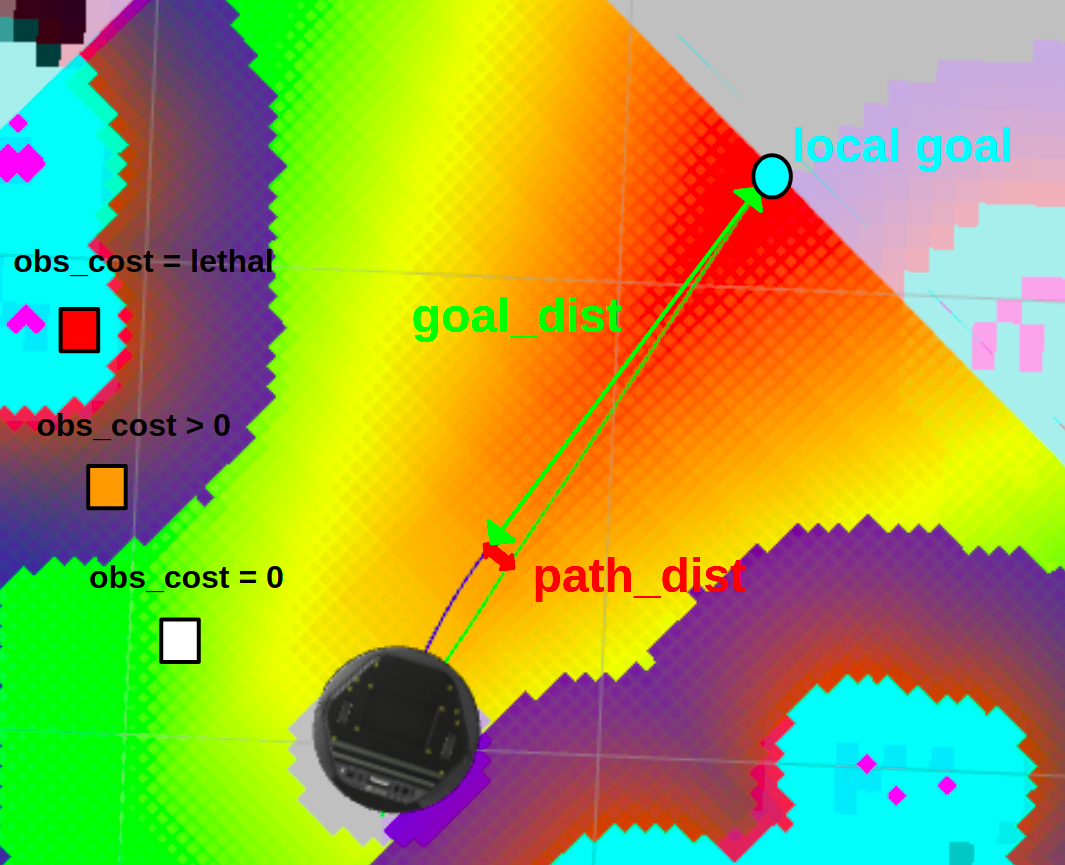
\includegraphics[scale=0.3]{cost_cloud.png}
    \caption{Cost cloud published in rviz. Red and green cells correspond to low and high cost respectively}
    \label{fig:my_label}
\end{figure}


Increasing \texttt{pdist\_scale} will make the robot stick more closely to the provided global plan, while increasing \texttt{gdist\_scale} will make the robot choose trajectories in which the end point is closer to the local goal. To make the robot more afraid of being close to obstacles increase \texttt{occdist\_scale}.

Since the trajectories are scored taking into account their endpoints, \texttt{sim\_time} will have a large effect on the behavior of the robot. Simulating to far ahead in the future  will result in smoother curves that are not very flexible. Setting this to 1-2 to seconds seems have good results in our case.

\subsubsection{Global and Local Costmap}
The global and local costmap value will influence the global and local plans created respectively so their parameters must be selected appropriately.
\paragraph{Main Parameters}
\begin{itemize}[label={}]
    \item \texttt{plugins} - Specifies the list of layers we want to use.
    \item \texttt{robot\_radius $(Hz)$} - The radius of the robot.
    \item \texttt{update\_frequency $(Hz)$} - Frequency at which the costmap updates itself.
    \item \texttt{height $(m)$} - height of the map.
    \item \texttt{width $(m)$} - width  of the map.
    \item \texttt{resolution $(m)$} - resolution  of the map.
    \item \texttt{transform\_tolerance $(s)$} - Maximum delay in transform (tf) data that is tolerable.
\end{itemize}

The plugins used by both global and local costmap are the \texttt{obstacle\_layer} and \texttt{inflation\_layer}. If we have a map that is being published we additionally  give the global costmap the  \texttt{static\_layer}.

The map sizes and resolution must be compromised with the update frequency to respect out limited computational resources.

\subsubsection{Obstacle layer}
This layer uses a list of sensors defined by the user to mark lethal obstacles on the costmap. It also raytraces obstacles in order to free up space.
\paragraph{Main Parameters}

\begin{itemize}[label={}]
    \item \texttt{observation\_sources} - Specifies the list of sensors we want to use to detect and/or clear obstacles.
    \item \texttt{obstacle\_range $(m)$} - maximum distance from the robot at which an obstacle will be inserted into the costmap.
    \item \texttt{raytrace\_range $(m)$} - distance to raytrace out obstacles from the map.
\end{itemize}

Increasing \texttt{raytrace\_range $(m)$} is useful when the costmap is cluttered with obstacles that need to be cleared. Otherwise if there are objects being cleared when they are not supposed to the parameter should be decreased.
\subsubsection{Inflation layer}
This layer takes into account lethal obstacles of the master costmap and sets the surrounding cells with a value that depends on the distance to the occupied cell.
\begin{itemize}[label={}]
    \item \texttt{cost\_scaling\_factor} - Exponential rate at which obstacle values are decreased in value.
    \item \texttt{inflation\_radius $(m)$} - The radius in meters to which the map inflates obstacle cost values.
\end{itemize}
\begin{align*}
    \textbf{cell value}=253*exp(-\texttt{cost\_scaling\_factor} * (\textbf{obsdist} - \textbf{insc\_radius}))
\end{align*}
The \texttt{cost\_scaling\_factor} and \texttt{inflation\_radius} parameters will determine how the values of the costmap are set and consequently  the navigation outputted plans. They must be tuned correctly so the robot avoid obstacles while still being able to go through narrow spaces.  


\section{Results}
Since the number of available parameters is so wide it is hard to admit a specific configuration as the most optimal one. However we find that the parameters shown in tables 1 and 2 give reasonable results when using both radar and lidar as sensor sources. 

\begin{center} 
\begin{adjustbox}{max width=\textwidth}
\begin{tabular}{ |c|l|c| } 
\hline
\makecell[c]{\textbf{Component}} & \makecell[c]{\textbf{Parameters}} & \textbf{Value} \\
\hline
 & base\_global\_planner   & navfn\\
\cline{2-3}
 & base\_local\_planner & TrajectoryPlanner\\
\cline{2-3}
Move Base & controller\_frequency   & 5.0 \\
\cline{2-3}
& controller\_patience  & 3.0\\
\cline{2-3}
 & planner\_frequency  & 1.0 \\
\cline{2-3}
 & planner\_patience  & 5.0 \\
 \hline
 & acc\_lim\_x    & 2.0 \\
\cline{2-3}
& acc\_lim\_y   & 0.0 \\
\cline{2-3}
& acc\_lim\_theta   & 2.0 \\
\cline{2-3}
& max\_vel\_x   & 0.4 \\
\cline{2-3}
& min\_vel\_x    & 0.1 \\
\cline{2-3}
& max\_vel\_theta    & 3.14 \\
\cline{2-3}
& min\_vel\_theta    & -3.14 \\
\cline{2-3}
TrajectoryPlanner & sim\_time   & 1.5 \\
\cline{2-3}
& sim\_granularity   & 0.025 \\
\cline{2-3}
& vx\_samples   & 3 \\
\cline{2-3}
& vtheta\_samples   & 20 \\
\cline{2-3}
& pdist\_scale   & 0.6 \\
\cline{2-3}
& gdist\_scale  & 0.4 \\
\cline{2-3}
& occdist\_scale  & 0.02 \\
\hline
Local \& Global Costmap  & robot\_radius  & 0.18 \\
\cline{2-3}
\hline
  & update\_frequency  & 20.0 \\
\cline{2-3}
 & rolling\_window  & true \\
\cline{2-3}
  Local & width  & 3.0 \\
\cline{2-3}
  Costmap  & height  & 3.0\\
\cline{2-3}
  & resolution  & 0.04 \\
\cline{2-3}
  & transform\_tolerance  & 0.5 \\
\hline
  & update\_frequency  & 15.0 \\
\cline{2-3}
 & rolling\_window  & true \\
\cline{2-3}
  Global & width  & 10.0 \\
\cline{2-3}
  Costmap  & height  & 10.0\\
\cline{2-3}
  & resolution  & 0.05 \\
\cline{2-3}
  & transform\_tolerance  & 0.5 \\
\hline

\end{tabular}
\end{adjustbox}
\captionof{table}{Navigation stack component parameters used in the test.} 

\end{center}
\begin{center}
\begin{adjustbox}{max width=\textwidth}
\begin{tabular}{ |c|c|l|c| } 
\hline
\makecell[c]{\textbf{Costmap}} & \makecell[c]{\textbf{Layer}}& \textbf{Parameter} & \textbf{Value} \\
\hline
&  & enabled & true \\
\cline{3-4}
 &  obstacle\_layer & obstacle\_range & 2.5 \\
\cline{3-4}
 &  & raytrace\_range & 3.0 \\
\cline{3-4}
 Global \& Local &  & observation\_sources & scan radar \\
\cline{2-4}
&  & enabled & true \\
\cline{3-4}
 & inflation\_layer & cost\_scaling\_factor & 5.0 \\
\cline{3-4}
 &  & inflation\_radius & 0.5 \\
\hline
Global  & static\_layer & enabled & true \\
\hline
\end{tabular}
\end{adjustbox}
\captionof{table}{Layers used in the global and local costmap and their parameter values used in this test.} 

\end{center}
\begin{comment}
There are three global planners currently available: \textbf{carrot\_planner}, \textbf{navfn} and \textbf{global\_planner}. In our case we will be using \textbf{navfn}.
%%DJAKTRA AND A* global plan image
%%RVIZ image
\paragraph{Main Parameters}
\begin{itemize}[label={}]
    \item \textbf{allow\_unknown} - Specifies whether or not to allow the planner to create plans that traverse unknown space (global costmap defines whether or not the goal is unknown space).
    \item \textbf{default\_tolerance} - A tolerance on the goal point for the planner.
\end{itemize}
%%NAV STACK IMG
\begin{figure}[!htb]
    \centering
    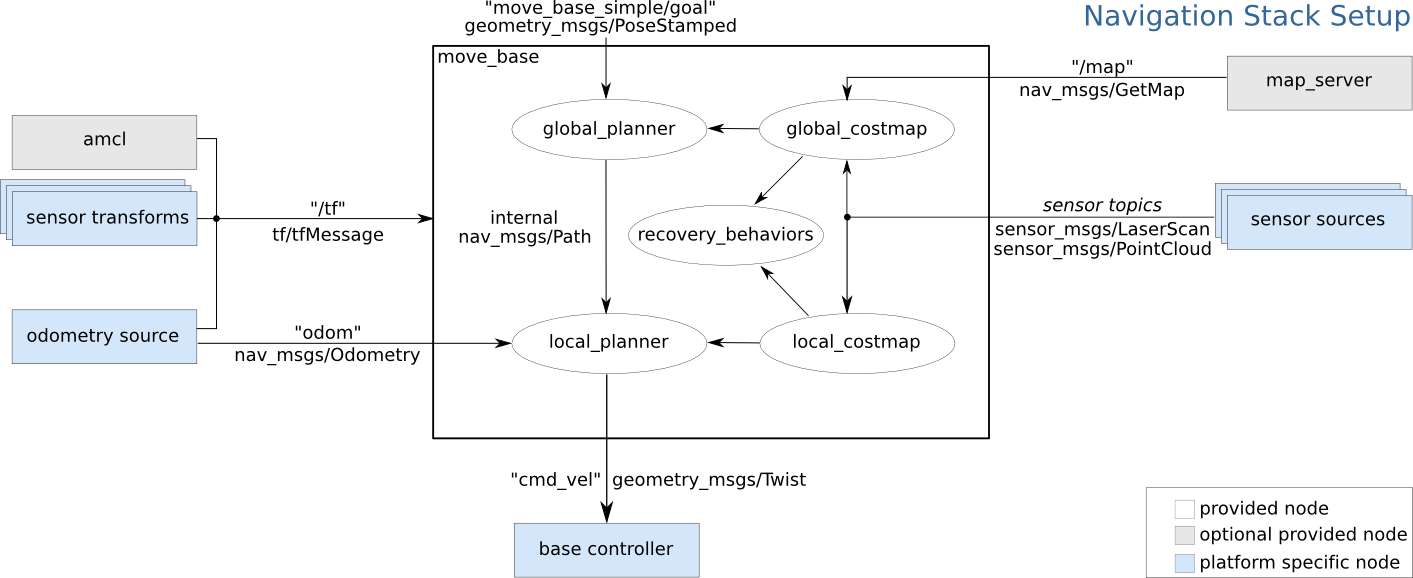
\includegraphics[width=\linewidth]{overview_tf.png}
    \caption{Clustering}
    \label{fig:my_label}
\end{figure}
\paragraph{Main Parameters}

After running various experiments in different conditions we conclude that the parameters shown in tables 1 and 2 of Appendix A make the robot achieve the goal quickly while still avoiding obstacles and minimizing the time it is stuck.

In this case we will choose \textbf{TrajectoryPlannerROS} as our local planner. This component has a large set of parameters that will determine how the robot will behave while navigating. The following like gives a brief overview over all of them:
\url{http://wiki.ros.org/base_local_planner#TrajectoryPlannerROS}
%%RVIZ costmap
\*
\section{Using the radar for autonomous navigation of the turtlebot}

\subsection{ROS Navigation stack setup}

The ROS navigation package offers a reliable way for a robot to navigate alone. In order to  do this it needs a sensor source to detect obstacles, a reliable source of odometry and optionally a mused . The map is used as global reference to the robot.
%%IMAGEM ROS NAVIGATION STACK
\subsubsection{ROS Navigation structure}
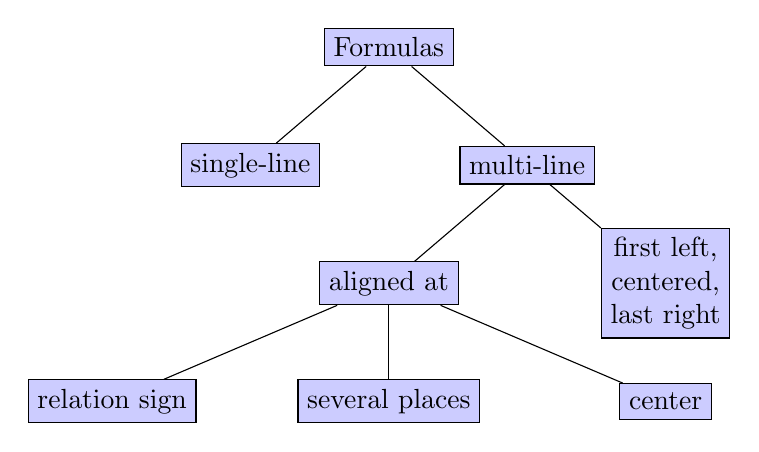
\begin{tikzpicture}[sibling distance=10em,
  every node/.style = {shape=rectangle, sharp corners,
    draw, align=center,
    top color=blue!20, bottom color=blue!20}]]
  \node {Formulas}
    child { node {single-line} }
    child { node {multi-line}
      child { node {aligned at}
        child { node {relation sign} }
        child { node {several places} }
        child { node {center} } }
      child { node {first left,\\centered,\\last right} } };
\end{tikzpicture}

In this case we will use the radar pointcloud and the lidar laserscan as sensor sources and amcl for localization.
\subsection{Results}

%RADAR CONCEPTS
\section{Radar basics}
In order to retrieve the best data for our application we first need to understand how the radar works. The following sections will try explain how the radar calculates the range, velocity and angle of an object.
\subsection{range Detection}
An FMCW radar transmits a signal called a “chirp”. A chirp is a sinusoid whose frequency  increases linearly with time.
%% put A t and f t plot
A chirp is characterized by a start frequency (fc), bandwidth(B) and duration (Tc). The slope (S) of the chirp is the rate at witch the frequency of the chirp increases and is given by:
\begin{equation}
    S=\frac{B}{T_c}
\end{equation}
%%PUT SOME TEXT
Object detection follows this steps:
\begin{enumerate}
    \item The chirp is transmitted by the TX antenna
    \item The chirp is reflected off an object and the reflected chirp is received at the RX antenna
    \item The RX signal and TX signal are ‘mixed’ and the resulting signal is called an ‘IF signal’
\end{enumerate}


%%PUT IMAGE
%%%When the transmitted chirp encounters an object it will reflect back to the radar and will be captured by the RX antenna.
The RX signal is a sum of delayed versions of the TX signal. This means that the resulting IF signal will be a combination of sinusoids. Each of this correspond to a reflection of an object. For object $i$ the corresponding frequency $f_i$ is equal to:
\begin{equation}
    f_i=S\tau_i
\end{equation}
Where $\tau_i$ is equal to the round trip delay of the wave and is equal to:
\begin{equation}
    \tau_i=\frac{2d_i}{c}
\end{equation}
Where $d_i$ corresponds to the distance of the object to the radar and $c$ the speed of light.
%% PUT image
Putting this together the distance of object $i$ is given by:
\begin{equation}
    d_i=\frac{f_ic}{2S}
\end{equation}
\subsection{range resolution}
\subsection{velocity Detection}
\subsection{angle Detection}

 %A cluster is just a subset of points of the cloud that are close together. This takes into account if a point has alot of close neighbours. If it has than it is considered a cluster.  
 \begin{figure}[!htb]
    \centering
    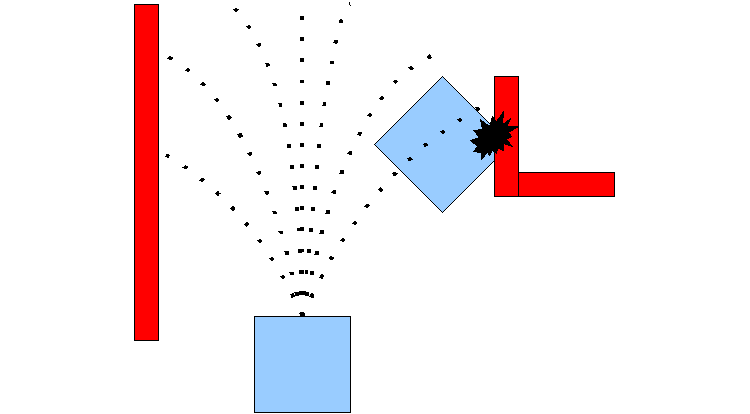
\includegraphics[width=\linewidth]{local_plan.png}
    \caption{Clustering}
    \label{fig:my_label}
\end{figure}
To start receiving the radar data and visualize it on the published PointCloud2 message using rviz by following this steps:
\begin{enumerate}
    \item Create your ROS workspace.
    %??? Anexo
    \item Install the serial ROS package and TI mmWave ROS Driver in that workspace.
    %??? Anexo
    \item  Finnaly, while in your workspace directory run the commands:
    \begin{lstlisting}[language=bash]
source devel/setup.bash
roslaunch ti_mmwave_rospkg rviz_1642_2d.launch
\end{lstlisting}
After setting up the necessary components (anexo 2) you can  start receiving and visualizing the radar data by running the following commands while in your ROS workspace directory:
 \begin{lstlisting}[language=bash]
source devel/setup.bash
roslaunch ti_mmwave_rospkg rviz_1642_2d.launch
\end{lstlisting}
This will launch the TI mmWave ROS Driver nodes that configure the EVM and publish the radar data. After that rviz will load and you should be able to visualize the objects detected by the radar. Figure \ref{fig:radar_rviz} shows an example of the radar data displayed on rviz. The points correspond to object detected by the radar.
\end{enumerate}
\end{comment}
\end{document}